\chapter{Tecnologie e strumenti utilizzati}\label{cap:Tecnologie e strumenti utilizzati}
Per il raggiungimento degli obiettivi del progetto di stage sono state utilizzate diverse tecnologie e strumenti. 
In questa sezione verranno riepilogate con una breve descrizione del loro utilizzo. 
\section{Linguaggi utilizzati}
\subsection{YAML}
YAML, acronimo di YAML Ain't Markup Language, è un linguaggio di Markup, noto per la sua leggibilità e la sua 
chiarezza espressiva. \\
La prima idea attorno al linguaggio YAML nasce attorno agli anni '90 quando Clark C. Evans, software developer, lo propone come alternativa a XML.\\
Nel 2001 Evans pubblica la prima specifica del linguaggio, che va a definire i principi fondamentali del linguaggio.\\
Negli anni YAML ha acquisito sempre più popolarità e interesse di utilizzo, in quanto ha offerto una configurazione semplice e leggibile 
per strumenti si DEVOPS, orchestrazione, automazione e molto altro (Figura \ref{fig:yaml}).\\
La storia di YAML è strettamente legata alla esigenza di semplificare la rappresentazione di dati complessi, 
in un formato più comprensibile a un essere umano e a macchine.\\
\begin{figure}[hpp]
    \centering
    
\includegraphics[width=0.5\textwidth]{images/tecnologie/logo_yaml.png}
    \caption{Logo di YAML}
    \label{fig:yaml}
\end{figure}
\pagebreak
\subsection{Python}
Python è un linguaggio di programmazione ad alto livello, orientato agli oggetti,
che si distingue per la sua sintassi chiara e intuitiva (Figura \ref{fig:python}).\\
Creato da Guido van Rossum e rilasciato per la prima volta nel 1991, è cresciuto fino a 
diventare uno dei linguaggi più utilizzati al mondo.\\
Data la sua semplicità e la sua versatilità, Python è utilizzato in diversi ambiti dallo sviluppo web, alla \gls{Data Analytics}{}, allo sviluppo di applicazione 
desktop e mobile, fino ad arrivare all'automazione e all'intelligenza artificiale.\\
\begin{figure}[hpp]
    \centering
    
\includegraphics[width=0.5\textwidth]{images/tecnologie/logo_python.png}
    \caption{Logo di Python}
    \label{fig:python}
\end{figure}
\section{Tecnologie utilizzate}
\subsection{Metodologia di sviluppo e strumenti di gestione di progetto}
Perseguendo la metodologia utilizzata da Sync Lab, il progetto di stage è stato sviluppato seguendo un
approccio \gls{agile}{}, simil \gls{Scrum}{} insieme a un \gls{modello incrementale}{}.\\ 
Come risultato di tutto ciò, il carico di lavoro pianificato, suddiviso in task, è stato distribuito in più incrementi successivi, 
chiamati \gls{sprint}{}.\\
Come prima operazione sono state definite le attività da svolgere e inserite all'interno del \gls{Product Backlog}{} e in seguito 
sono state pianificate all'interno di ogni \gls{sprint}{}.\\
L'adozione di tale metodologia di sviluppo, la si ritiene una scelta vincente, in quanto ha permesso di avere un'idea chiara
delle attività da svolgere e di avere un'idea chiara dei tempi di sviluppo. Inoltre ha permesso quanto prima di ottenere 
parti del prototipo funzionanti, che hanno permesso di avere un feedback da parte del tutor aziendale.\\
Per quanto riguarda il \gls{modello incrementale}{}, il maggiore vantaggio ottenuto è stato la metodologia di sviluppo: le componenti 
con maggiore priorità sono state sviluppate per prime, perchè hanno fornito la base su cui sviluppare le componenti successive. Ciò significa che 
le funzionalità essenziali del prototipo sono state disponibili sin da subito e sono state migliorate e ampliate con il progredire dello sviluppo del progetto.
\subsubsection{ClickUp}   %strumento di issue tracking system utilizzato
\textbf{ClickUp} (Figura \ref{fig:clickup}) è lo strumento di project management utilizzato per la gestione del progetto di stage.\\ 
È una piattaforma cloud che offre strumenti e funzionalità per la gestione di attività in modo efficente.\\
Presenta una interfaccia intuitiva e semplice da utilizzare, che permette di gestire le attività in modo semplice e veloce.\\
\pagebreak
\\
Offre la possibilità di creare \gls{board}{} personalizzate, in cui inserire le attività da svolgere, e di creare \gls{task}{} personalizzati,
permette di dare priorità alle attività, di assegnarle a un membro del team e d'impostare una data di scadenza.\\

\begin{figure}[h]
    \centering
    
\includegraphics[width=0.4\textwidth]{images/tecnologie/logo_clickup.png}
    \caption{Logo di ClickUp}
    \label{fig:clickup}
\end{figure}
\subsection{Ambiente di sviluppo}

\subsubsection{Docker Compose}
Docker Compose (Figura \ref{fig:docker_compose}) è uno strumento che permette di definire e gestire applicazioni \gls{Docker}{} multi-container. \\
Utilizza il linguaggio YAML per configurare i servizi dell'applicazione e fornisce un'interfaccia da riga di comando per la gestione dei \gls{container}{}.\\
Docker Compose permette di definire ed avviare più \gls{container}{} \gls{Docker}{} in modo coordinato, risolvendo 
la sfida dell'orchestrazione dei \gls{container}{}.\\
Mentre \gls{Docker}{} permette di definire singoli \gls{container}{}, Docker Compose estende queste funzionalità permettendo agli sviluppatori 
di definire in modo dichiarativo, oltre ai servizi contenuti in ogni applicazione, anche le relazioni tra i \gls{container}{} e le configurazioni di rete, volumi e variabili d'ambiente.\\
\begin{figure}
    \centering
    
\includegraphics[width=0.4\textwidth]{images/tecnologie/logo_docker_compose.png}
    \caption{Logo di Docker Compose}
    \label{fig:docker_compose}
\end{figure}
\pagebreak
\subsection{Versioning}
\subsubsection{Git}
\textbf{Git} è un sistema di controllo versione distribuito, utilizzato per il tracciamento delle modifiche ai file di un progetto.\\ 
Creato da Linus Torvalds nel 2005, GIT è stato pensato per la gestione del codice sorgente del kernel Linux, ma è stato adottato 
per progetti di ogni genere, di piccole e grandi dimensioni (Figura \ref{fig:git}).\\
\begin{figure}[hpp]
    \centering
    
\includegraphics[width=0.4\textwidth]{images/tecnologie/logo_git.png}
    \caption{Logo di Git}
    \label{fig:git}
\end{figure}

\noindent È uno dei sistemi di controllo di versione più utilizzati al mondo, grazie alla sua velocità, alla sua efficienza e alla sua flessibilità.\\
Come tutti i sistema di controllo di versione si basa sul concetto di \gls{repository}{}, ovvero un archivio contenente i file e tutti i 
\gls{metadati}{} relativi alle modifiche effettuate.\\  
In \textbf{Git} un file può trovarsi in tre stati diversi: \textit{commited} (versionati), \textit{modified} (modificati) e \textit{staged} (pronti per essere versionati).\\
Ogni nuovo modifica, se versionata all'interno del \gls{repository} viene identificata da un \textit{commit}, avente un identificativo univoco di 40 caratteri. Modificato 
significa che il file è stato modificato ma non è ancora stato versionato, mentre staged significa che il file è stato modificato e preparato per essere inserito nel 
prossimo \textit{commit}.\\
Quanto detto illustra le operazioni essenziali che possono essere effettuate con \textbf{Git} (Figura \ref{fig:git_workflow}).
\begin{figure}[hpp]
    \centering
    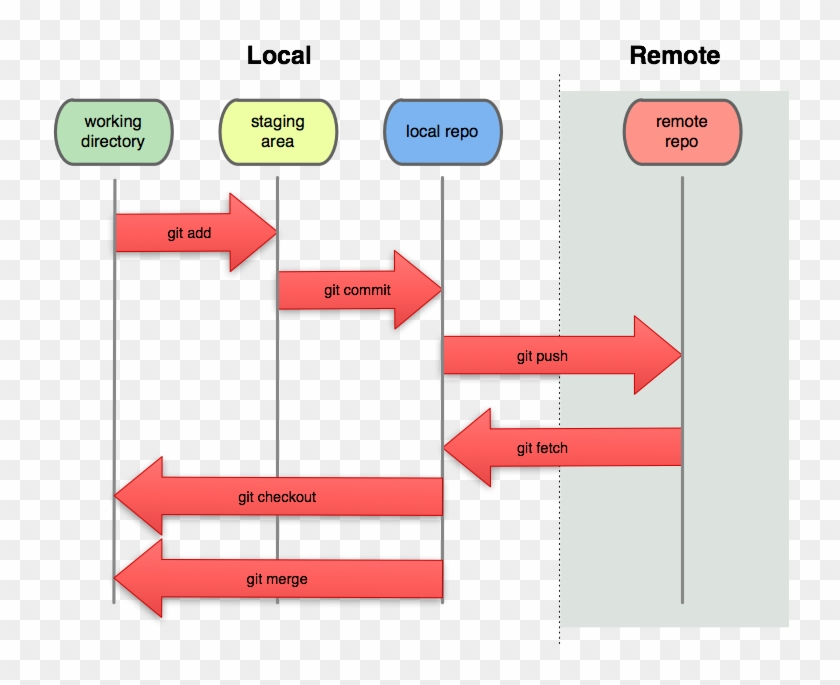
\includegraphics[width=0.5\textwidth]{images/tecnologie/comandi_git.png}
    \caption{Comandi di base di Git}
    \label{fig:git_workflow}
\end{figure}
Essenzialmente un workflow di bse con \textbf{Git} prevede:
\begin{list}{-}{}
    \item \textbf{Clonare} un \gls{repository}{}, se già esistente;
    \item \textbf{Modificare} i file all'interno della \gls{working directory}{};
    \item \textbf{Stage} dei file, ovvero prepararli per il prossimo \textit{commit}, aggiungendoli alla \textit{staging area} con il comando \textit{git add};
    \item \textbf{Commit} dei file, ovvero versionarli, con il comando \textit{git commit}, i file così come son salvati nella \textit{staging area} vengono versionati all'interno del \gls{repository}{};
    \item \textbf{Push} delle modifiche sul \gls{repository}{} remoto.
\end{list}
\subsubsection{GitHub}
Per quanto riguarda il servizio di hosting che ha ospita il \gls{repository}{} remoto è stato utilizzato \textbf{GitHub}, andando a condividere 
i contenuti tra il mio account e quello del tutor aziendale (Figura \ref{fig:github}).\\
\begin{figure}[hpp]
    \centering
    
\includegraphics[width=0.4\textwidth]{images/tecnologie/logo_github.png}
    \caption{Logo di GitHub}
    \label{fig:github}
\end{figure}
\\
\textbf{GitHub} è una piattaforma di hosting per progetti software, che utilizza \textbf{Git} come sistema di controllo di versione e contiene tutti 
i file e i \gls{metadati}{} relativi alle modifiche validate lungo le fasi del progetto.\\
\pagebreak
\subsection{Documentazione}
Per quanto riguarda la redazione della documentazione, Sync Lab non ha uno standard prefissato e mi ha permesso di scegliere quale software utilizzare per la 
produzione dei documenti. La scelta è ricaduta su \textbf{LaTeX}, un linguaggio di markup per la preparazione di testi.\\
\subsubsection{LaTeX}
\textbf{LaTex}  è un sistema di composizione tipografica ampiamente utilizzato per la creazione di documenti di alta qualità. A differenza dei tradizionali editor di testo, LaTeX si basa su comandi di formattazione e struttura, consentendo agli utenti di concentrarsi sul contenuto del documento anziché sul suo aspetto visivo.\\
È stato sviluppato da Leslie Lamport negli anni '80 come estensione di TeX, un linguaggio e motore di composizione sviluppati da Donald Knuth (Figura \ref{fig:latex}).

\noindent \textbf{LaTeX} semplifica notevolmente la creazione di documenti complessi, grazie alla sua capacità di gestire automaticamente numerazione delle sezioni, citazioni bibliografiche, tabelle dei contenuti e molte altre funzionalità tipografiche avanzate.
L'ecosistema che \textbf{LaTeX} offre una vasta gamma di pacchetti e stili predefiniti che consentono di creare documenti sofisticati e professionali.
Per quanto riguarda la scelta dell'editor da utilizzare l'azienda non ha dato vincoli rilevanti, quindi la scelta è ricaduta su \textbf{TexLive}, un distribuzione \textbf{LaTeX} per sistemi operativi Linux e su \textbf{Texworks} come editor di testo.
\begin{figure}[hpp]
    \centering
    
\includegraphics[width=0.3\textwidth]{images/tecnologie/logo_latex.png}
    \caption{Logo di LaTeX}
    \label{fig:latex}
\end{figure}

\newpage
\pagestyle{empty}
\null % o \mbox{} o \phantom{X}
\newpage